\documentclass[10pt]{article}
% PNAS version (Research Report, Social Sciences / Economic Sciences; secondary: Psychological and Cognitive Sciences).
% PNAS has a format-neutral policy for initial submissions: this file follows the PNAS structure (abstract <= 250 words,
% significance statement <= 120 words, untitled introduction, Results, Discussion, Materials and Methods, numbered references,
% ~6 pages / ~4,000 words, 3 display items); after acceptance, transfer the text into the official PNAS LaTeX template (Overleaf).
% Submission track: Direct Submission.
% Supporting information: wellbeing_pnas_si.tex (SI Appendix). Compile from papers/, twice each:
%   latexmk -pdf -outdir=build wellbeing_pnas.tex ; latexmk -pdf -outdir=build wellbeing_pnas_si.tex
% References to the SI Appendix (Table S1, S3...) are written as plain numbers so that this file compiles on its own:
% update them if the order of tables in wellbeing_pnas_si.tex changes.
\usepackage[T1]{fontenc}
\usepackage[utf8]{inputenc}
\usepackage{mathpazo}
\usepackage[margin=2cm]{geometry}
\usepackage[numbers,round,sort&compress]{natbib}
\usepackage{graphicx, booktabs, adjustbox, amsmath, amssymb, xcolor, caption, lineno}
\captionsetup{font=small, labelfont=bf}
\usepackage[colorlinks=true, urlcolor=purple, linkcolor=blue, citecolor=violet]{hyperref}
\usepackage{xspace}
\xspaceaddexceptions{]\%}
\newcommand{\corGallupWHR}{0.993\xspace}
\newcommand{\corGallupWHRoldMapping}{0.89\xspace}
\newcommand{\nGallupCountryYears}{2351\xspace}
\newcommand{\nGallupCountries}{168\xspace}
\newcommand{\nWVSCountryYears}{304\xspace}
\newcommand{\nWVSCountries}{108\xspace}
\newcommand{\nWVSRespondents}{439531\xspace}
\newcommand{\nFabre}{11000\xspace}
\newcommand{\nFabreCountries}{10\xspace}
\newcommand{\bestIncome}{Cluster k=7 nominal\xspace}
\newcommand{\shareRegionBetterWVS}{86\xspace}
\newcommand{\shareRegionBetterWVSbest}{79\xspace}
\newcommand{\nSpecsWVS}{952\xspace}
\newcommand{\meanShareIncomeBest}{28\xspace}
\newcommand{\meanRtwoIncomeBest}{19\xspace}
\newcommand{\meanRtwoIncomePPP}{12\xspace}
\newcommand{\meanRtwoRegion}{37\xspace}
\newcommand{\RtwoSatisfiedMeanPPP}{20\xspace}
\newcommand{\RtwoHappinessMeanPPP}{4\xspace}
\newcommand{\RtwoVeryHappyPPP}{0\xspace}
\newcommand{\shareRegionBetterGallup}{35\xspace}
\newcommand{\shareIncomeGallupMean}{60\xspace}
\newcommand{\RtwoGallupMeanPPP}{61\xspace}
\newcommand{\RtwoGallupRegion}{48\xspace}
\newcommand{\RtwoWHRPPP}{63\xspace}
\newcommand{\RtwoWHRRegion}{55\xspace}
\newcommand{\shareRegionBetterNoLatamEE}{27\xspace}
\newcommand{\shareIncomeNoLatamEE}{34\xspace}
\newcommand{\shareRegionBetterContinents}{54\xspace}
\newcommand{\shareRegionBetterWB}{64\xspace}
\newcommand{\cvIncomeSatisfiedMean}{0.18\xspace}
\newcommand{\cvRegionSatisfiedMean}{0.44\xspace}
\newcommand{\cvIncomeGallupMean}{0.60\xspace}
\newcommand{\cvRegionGallupMean}{0.45\xspace}
\newcommand{\shareCvRegionBetterWVS}{100\xspace}
\newcommand{\corHappySatisfied}{0.72\xspace}
\newcommand{\corHappinessSatisfactionMean}{0.76\xspace}
\newcommand{\corVeryHappySatisfiedMean}{0.63\xspace}
\newcommand{\slopeVeryHappy}{0.005\xspace}
\newcommand{\pVeryHappy}{0.85\xspace}
\newcommand{\happiestFirst}{Switzerland\xspace}
\newcommand{\happiestFirstN}{10\xspace}
\newcommand{\happiestSecond}{Mexico\xspace}
\newcommand{\happiestSecondN}{9\xspace}
\newcommand{\happiestThird}{Kyrgyzstan\xspace}
\newcommand{\happiestThirdN}{6\xspace}
\newcommand{\happiestRegionWestern}{24\xspace}
\newcommand{\happiestRegionLatinAmerica}{19\xspace}
\newcommand{\happiestRegionAsia}{16\xspace}
\newcommand{\happiestRegionAfrica}{5\xspace}
\newcommand{\nHappiestCells}{64\xspace}
\newcommand{\treeRegionFirst}{8\xspace}
\newcommand{\withinRtwoSatisfiedMean}{0.22\xspace}
\newcommand{\withinSlopeSatisfiedMean}{1.68\xspace}
\newcommand{\crossSlopeSatisfiedMean}{1.09\xspace}
\newcommand{\withinSlopeVeryHappy}{0.18\xspace}
\newcommand{\pWithinVeryHappy}{0.004\xspace}
\newcommand{\nWithin}{272\xspace}
\newcommand{\RtwoFreedomSatisfaction}{63\xspace}
\newcommand{\shapleyFreedom}{40\xspace}
\newcommand{\shapleyFreedomRegion}{26\xspace}
\newcommand{\shapleyFreedomIncome}{9\xspace}
\newcommand{\RtwoTolerance}{21\xspace}
\newcommand{\RtwoGod}{0\xspace}
\newcommand{\RtwoGrowth}{2\xspace}
\newcommand{\nonresponseSatisfactionWVS}{1.5\xspace}
\newcommand{\nonresponseHappinessWVS}{1.7\xspace}
\newcommand{\corNonresponseGDP}{-0.08\xspace}
\newcommand{\effectLadder}{-0.45\xspace}
\newcommand{\seLadder}{0.05\xspace}
\newcommand{\effectScale}{0.14\xspace}
\newcommand{\seScale}{0.05\xspace}
\newcommand{\effectLadderZeroTen}{-0.46\xspace}
\newcommand{\effectScaleZeroTen}{-0.26\xspace}
\newcommand{\effectLadderSatisfied}{-9\xspace}
\newcommand{\interactionLadderIncome}{-0.004\xspace}
\newcommand{\pInteractionLadderIncome}{0.92\xspace}
\newcommand{\gradientIncomeSatisfaction}{0.69\xspace}
\newcommand{\pHeterogeneityWording}{0.000\xspace}
\newcommand{\chiHeterogeneityWording}{93.4\xspace}
\newcommand{\wordingCHE}{-0.34\xspace}
\newcommand{\wordingDEU}{-0.53\xspace}
\newcommand{\wordingESP}{-1.12\xspace}
\newcommand{\wordingFRA}{-0.50\xspace}
\newcommand{\wordingGBR}{-0.63\xspace}
\newcommand{\wordingITA}{-0.55\xspace}
\newcommand{\wordingJPN}{0.36\xspace}
\newcommand{\wordingPOL}{-0.55\xspace}
\newcommand{\wordingSAU}{-0.79\xspace}
\newcommand{\wordingUSA}{-0.63\xspace}
\newcommand{\wordingMin}{-1.12\xspace}
\newcommand{\wordingMax}{0.36\xspace}
\newcommand{\decompMeanGap}{-0.39\xspace}
\newcommand{\decompMeanQuestion}{-0.71\xspace}
\newcommand{\decompMeanResidual}{0.32\xspace}
\newcommand{\decompShareLevelQuestion}{1.83\xspace}
\newcommand{\decompVarShareQuestion}{-0.20\xspace}
\newcommand{\decompVarShareResidual}{1.20\xspace}
\newcommand{\decompMeanAbsGap}{0.43\xspace}
\newcommand{\decompMeanAbsResidual}{0.64\xspace}
\newcommand{\decompRmsePredictionGallup}{0.73\xspace}
\newcommand{\decompRmseNaive}{0.42\xspace}
\newcommand{\decompMeanGapSat}{-0.05\xspace}
\newcommand{\decompMeanQuestionSat}{-0.11\xspace}
\newcommand{\decompVarShareQuestionSat}{-0.11\xspace}
\newcommand{\decompSdGap}{0.44\xspace}
\newcommand{\decompSdQuestion}{0.45\xspace}
\newcommand{\decompSdResidual}{0.69\xspace}
\newcommand{\decompCorGapQuestion}{-0.20\xspace}
\newcommand{\decompLowMeanGap}{-0.44\xspace}
\newcommand{\decompHighMeanGap}{-0.34\xspace}
\newcommand{\decompLowMeanQuestion}{-0.85\xspace}
\newcommand{\decompHighMeanQuestion}{-0.56\xspace}
\newcommand{\decompLowMeanResidual}{0.17\xspace}
\newcommand{\decompHighMeanResidual}{0.46\xspace}
\newcommand{\decompLowVarShareQuestion}{-0.52\xspace}
\newcommand{\decompHighVarShareQuestion}{0.15\xspace}
\newcommand{\decompLowShareLevelQuestion}{1.42\xspace}
\newcommand{\decompHighShareLevelQuestion}{2.27\xspace}
\newcommand{\decompLowCorGapQuestion}{-0.47\xspace}
\newcommand{\decompHighCorGapQuestion}{0.14\xspace}
\newcommand{\nDecompCountries}{10\xspace}
\newcommand{\nSameYear}{7\xspace}
\newcommand{\nRecent}{4\xspace}
\newcommand{\varShareQuestionSameYear}{-0.27\xspace}
\newcommand{\varShareQuestionRecent}{-0.81\xspace}
\newcommand{\shareLevelQuestionSameYear}{1.60\xspace}
\newcommand{\shareLevelQuestionRecent}{1.19\xspace}
\newcommand{\meanSampleEffectGallup}{0.75\xspace}
\newcommand{\corFabreWHR}{0.75\xspace}
\newcommand{\minSampleEffectGallup}{0.16\xspace}
\newcommand{\maxSampleEffectGallup}{1.24\xspace}
\newcommand{\meanSampleEffectWVS}{0.54\xspace}
\newcommand{\meanFabreGallupZero}{5.93\xspace}
\newcommand{\meanFabreWVSOne}{6.64\xspace}
\newcommand{\sampleEffectUSWVS}{0.49\xspace}
\newcommand{\nCommon}{149\xspace}
\newcommand{\nCommonCountries}{83\xspace}
\newcommand{\RtwoCommonGallup}{0.49\xspace}
\newcommand{\RtwoCommonWVS}{0.11\xspace}
\newcommand{\slopeCommonGallup}{1.76\xspace}
\newcommand{\slopeCommonWVS}{0.77\xspace}
\newcommand{\slopeGapGDP}{1.07\xspace}
\newcommand{\seSlopeGapGDP}{0.16\xspace}
\newcommand{\RtwoGapGDP}{0.31\xspace}
\newcommand{\slopeQuestionGDP}{0.30\xspace}
\newcommand{\seSlopeQuestionGDP}{1.75\xspace}
\newcommand{\RtwoAdjustedWVS}{0.20\xspace}
\newcommand{\shareIncomeCommonGallup}{51\xspace}
\newcommand{\shareIncomeCommonWVS}{15\xspace}

\bibliographystyle{unsrtnat}
\renewcommand{\thetable}{\arabic{table}}

\title{Whether richer countries are happier depends on the survey}
% Alternative titles: "Survey question and sample shape the cross-country link between income and well-being";
% "Region predicts national well-being better than income, unless you ask Gallup"
\author{Adrien Fabre\\ \small CNRS, CIRED, % (Centre international de recherche sur l'environnement et le d\'eveloppement), 
Paris, France. \href{mailto:adrien.fabre@cnrs.fr}{adrien.fabre@cnrs.fr}. ORCID: \href{https://orcid.org/0000-0001-5245-7772}{0000-0001-5245-7772}}
\date{}

\begin{document}
\maketitle
\linenumbers

\noindent\textbf{Classification:} Social Sciences (Economic Sciences). \textbf{Keywords:} subjective well-being $|$ GDP $|$ world regions $|$ survey methodology $|$ question wording

\begin{abstract}
\noindent Across countries, average life evaluations rise with the logarithm of GDP per capita, a stylized fact that underpins the view that growth brings happiness. I show that this relationship depends on the survey. In the World Values Survey (WVS, 1981--2023, \nWVSCountries countries), log GDP per capita explains on average \meanRtwoIncomePPP\% of the cross-country variance of eight well-being indicators, less than a country's broad world region (\meanRtwoRegion\%), which predicts better in and out of sample. In the Gallup World Poll (\nGallupCountries countries), income predicts life evaluations as well as region. The two surveys differ in their question (Cantril ladder vs.\ life satisfaction) and in their samples. To separate the two, I randomized the question wording and scale in an online survey of \nFabre respondents in ten high-income countries. Asked to the same respondents, the ladder is better predicted by GDP than life satisfaction ($R^2$ of \RtwoTenFabreLadderPooled vs.\ \RtwoTenFabreSatisfactionPooled across countries), which reproduces about half of the difference in predictive capacity between Gallup and the WVS in these countries (\RtwoTenGallup vs.\ \RtwoTenWVS). Yet both questions yield income gradients as steep as Gallup's, three times steeper than the WVS's: life satisfaction adds country-specific deviations from the income gradient, while the flat WVS gradient stems from its samples. Wording and samples thus both shape the cross-country relation between income and well-being, which should be assessed across surveys and questions before informing policy.
\end{abstract}

\paragraph{Significance statement.} Rankings of the world's happiest countries and the belief that richer countries are happier rest mostly on one survey, the Gallup World Poll. In the other major cross-national survey, the World Values Survey, national income predicts well-being less well than a country's broad world region does. A survey experiment in ten countries shows that about half of this discrepancy comes from the question asked, and the rest from differences between survey samples. How strongly income predicts national well-being thus depends on how, and whom, one asks. Policies should target well-being directly rather than assume that growth delivers it, and cross-country evidence on well-being should be checked across surveys.

\section*{Introduction}

Which country is the happiest? The answer most often heard, based on the World Happiness Report, is a Scandinavian, high-income country. Behind this answer lies a robust stylized fact: across countries, average life evaluations increase with the logarithm of GDP per capita \citep{deaton_income_2008,stevenson_economic_2008,sacks_new_2012}. Using the Gallup World Poll, Deaton \citep{deaton_income_2008} found a correlation above 0.8 between average life evaluation and log GDP per capita. This correlation is frequently invoked to support the view that economic growth is a reliable route to higher well-being \citep{stevenson_economic_2008,jebb_happiness_2018}, against the Easterlin paradox \citep{easterlin_does_1974,easterlin_happiness_2010}.

Yet the two main sources of cross-national well-being data do not agree. Income is more strongly related to Gallup's Cantril ladder than to the life-satisfaction question of the World Values Survey (WVS), a difference that Deaton attributed partly to WVS samples in poor countries, which were ``mostly literate and urban'' \citep{deaton_income_2008}. The surveys differ both in their question and in their samples, so observational comparisons cannot tell which difference matters \citep{bjornskov_how_2010}. If it is the question, the two surveys measure different constructs---for instance, if the ``best possible life'' of the ladder evokes wealth and status \citep{nilsson_cantril_2024}, just as income is more closely related to life evaluations than to emotional well-being \citep{kahneman_high_2010}---and conclusions depend on which construct one cares about. If it is the samples, they measure the same construct with different errors.

This paper makes two contributions. First, it benchmarks the predictive capacity of GDP per capita against a very simple alternative, the country's world region, in both surveys. Latin America is known to be happier than its income would predict \citep{graham_paradox_2009,rojas_handbook_2016}, and post-communist countries unhappier \citep{guriev_unhappiness_2009}, but the predictive power of income and region has not been systematically compared. Second, it separates the effects of question and sample with a randomized survey experiment in ten countries, in which the question wording (ladder vs.\ satisfaction) and scale (0--10 vs.\ 1--10) vary across respondents of the same sample.

\section*{Results}

\subsection*{Income predicts national well-being less than region in the WVS, but not in Gallup}

In the WVS, complemented with the European Values Study (\nWVSCountryYears country-years, 1981--2023), the relation between GDP per capita and mean life satisfaction is positive but loose (Fig.~\ref{fig:scatter}A): countries with a GDP per capita around \$10,000 span most of the observed range of satisfaction, from Eastern Europe at the bottom to Latin America at the top. Log GDP per capita explains \RtwoSatisfiedMeanPPP\% of the variance of mean satisfaction, \RtwoHappinessMeanPPP\% of the variance of mean happiness (Fig.~\ref{fig:scatter}C), and essentially none of the share of ``very happy'' people. On average over eight indicators of national well-being, it explains \meanRtwoIncomePPP\% of the variance (95\% CI [\ciLowWVSMeanRIncome\%; \ciHighWVSMeanRIncome\%], bootstrap resampling countries), against \meanRtwoRegion\% ([\ciLowWVSMeanRRegion\%; \ciHighWVSMeanRRegion\%]) for a classification of countries into five world regions (SI Appendix, Table~S1).

Region has more parameters than log GDP, which could favor it in sample. I therefore also use six other income measures, including categorical ones with as many categories as regions: log GDP per capita at market exchange rates, sextiles of GDP per capita, and clusters of log GDP per capita obtained by $k$-means ($k = 5$, 6 or 7 at PPP; $k = 7$ at market exchange rates), which let the data choose income thresholds. The best of them (seven clusters at market exchange rates) explains \meanRtwoIncomeBest\% of the variance on average, still less than region. Out of sample, region also predicts better than income for every indicator: when each country is predicted by a model estimated on all other countries, the cross-validated $R^2$ of mean satisfaction is \cvRegionSatisfiedMean with region, against \cvIncomeSatisfiedMean with log GDP (SI Appendix, Table~S3). Decomposing the variance explained jointly by income and region with Shapley values, region is the better predictor in \shareRegionBetterWVS\% of \nSpecsWVS combinations of indicators, income measures and robustness specifications (SI Appendix, Table~S4). This advantage rests on Latin America and Eastern Europe: region remains the better predictor when either is excluded (\shareRegionBetterNoLatam\% and \shareRegionBetterNoEE\% of cases), but not when both are (\shareRegionBetterNoLatamEE\%; SI Appendix, Table~S5).

The Gallup World Poll tells a different story (Fig.~\ref{fig:scatter}B). In its latest observation for each of \nGallupCountries countries, log GDP explains \RtwoGallupMeanPPP\% of the variance of the mean ladder ([\ciLowGallupRIncome\%; \ciHighGallupRIncome\%]), against \RtwoGallupRegion\% for region ([\ciLowGallupRRegion\%; \ciHighGallupRRegion\%]), and income accounts for \shareIncomeGallupMean\% of the variance explained jointly with region. Region predicts better only for the upper tail of the distribution (shares answering 9 or 10), which, like the share of very happy people in the WVS, is almost unrelated to income.

\begin{figure*}[tbp]
    \centering
    \begin{minipage}{.49\textwidth}\small\textit{A}\\ 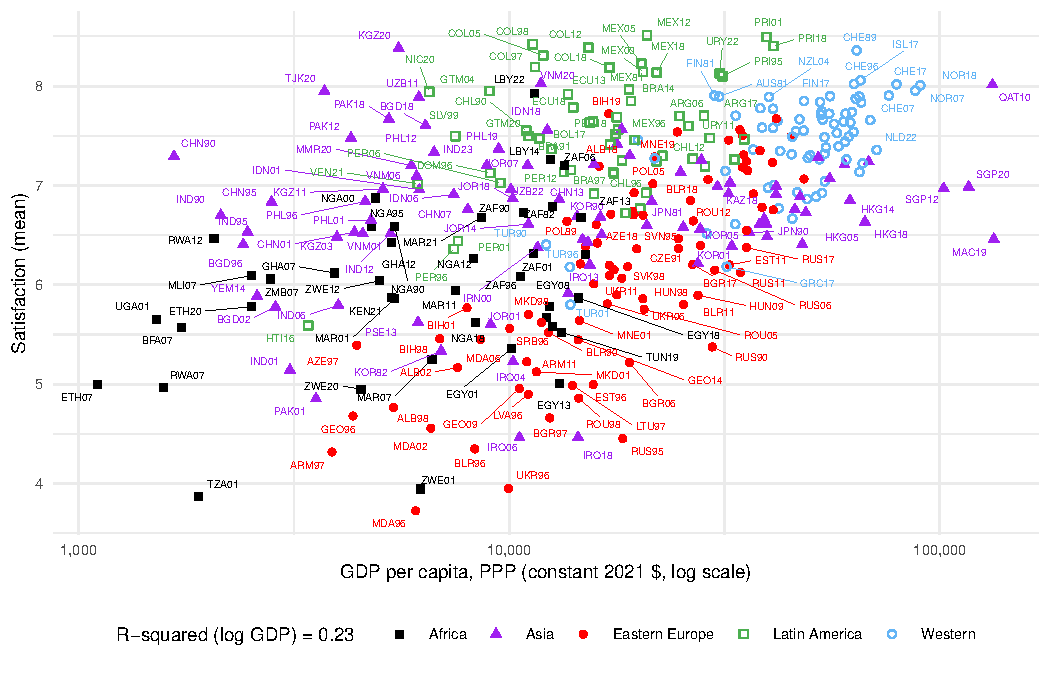
\includegraphics[width=\textwidth]{../figures/main/wvs_satisfied_mean_vs_gdp_ppp.pdf}\end{minipage}\hfill
    \begin{minipage}{.49\textwidth}\small\textit{B}\\ 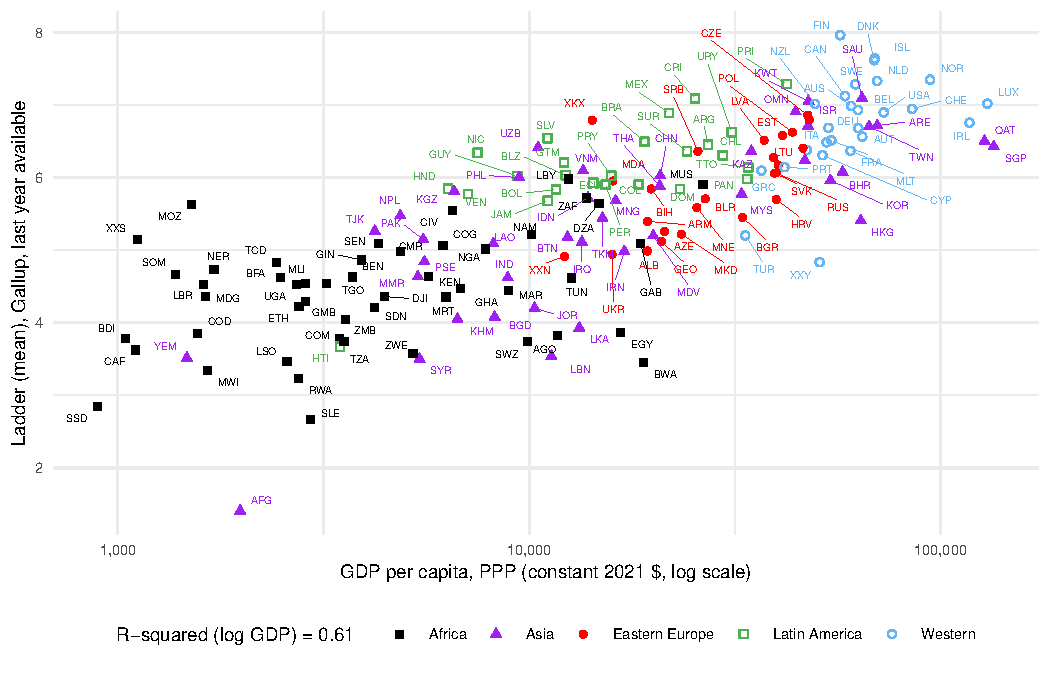
\includegraphics[width=\textwidth]{../figures/main/gallup_ladder_mean_vs_gdp_ppp.pdf}\end{minipage}\\[1ex]
    \begin{minipage}{.49\textwidth}\small\textit{C}\\ 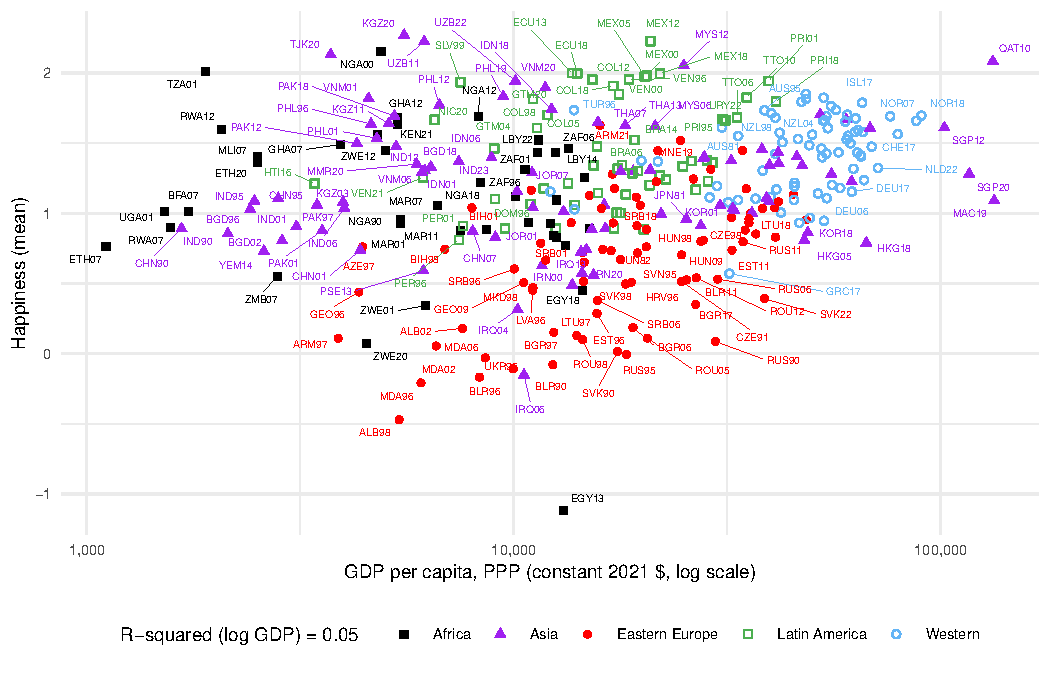
\includegraphics[width=\textwidth]{../figures/main/wvs_happiness_mean_vs_gdp_ppp.pdf}\end{minipage}\hfill
    \begin{minipage}{.49\textwidth}\small\textit{D}\\ 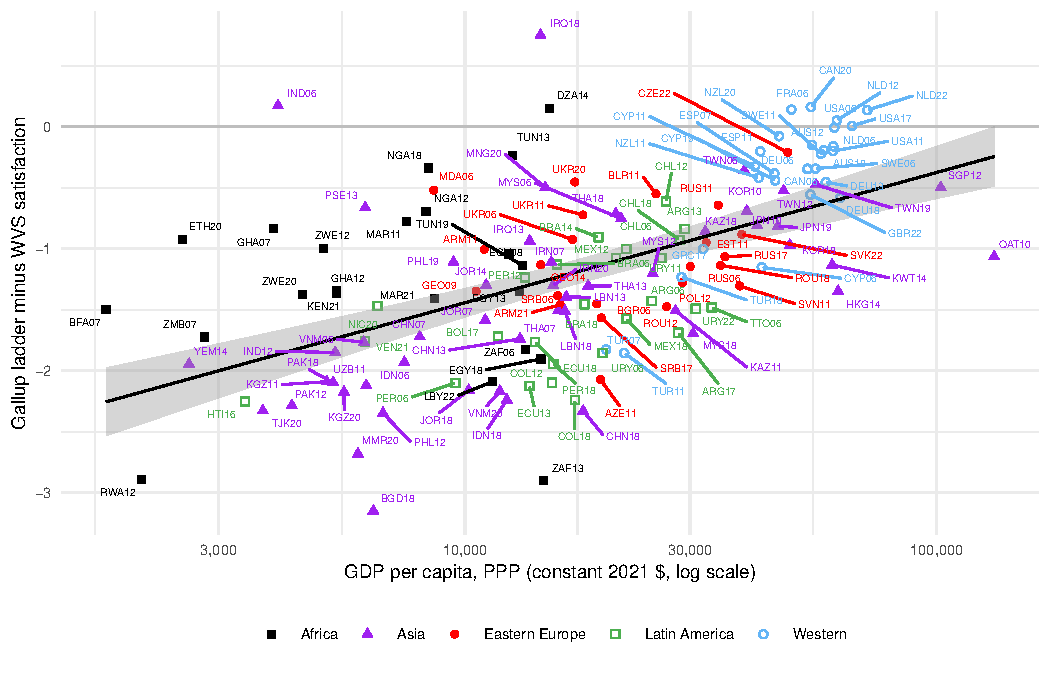
\includegraphics[width=\textwidth]{../figures/main/gap_gallup_wvs_vs_gdp.pdf}\end{minipage}
    \caption{National well-being and GDP per capita (PPP, log scale). (\textit{A}) Mean life satisfaction (1--10), WVS/EVS, \nWVSCountryYears country-years, 1981--2023 (labels: country code and year). (\textit{B}) Mean Cantril ladder (0--10), Gallup World Poll, latest observation for each of \nGallupCountries countries (2006--2023). (\textit{C}) Mean happiness, WVS/EVS (answers coded $+3$, $+1$, $-1$, $-3$ from \textit{Very happy} to \textit{Not at all happy}). (\textit{A}--\textit{C}) Colors and shapes: world regions; legends give the $R^2$ of the regression on log GDP per capita. (\textit{D}) Mean WVS life satisfaction minus mean Gallup ladder in the same country-year, \nCommon country-years observed by both surveys; line: OLS fit with 95\% confidence band.}\label{fig:scatter}
\end{figure*}

\subsection*{The discrepancy is largest in low-income countries}

The discrepancy is not due to different country coverage. In the \nCommon country-years observed by both surveys, log GDP explains \RtwoCommonGallup of the variance of Gallup's mean ladder but \RtwoCommonWVS of WVS mean satisfaction, and income accounts for \shareIncomeCommonGallup\% of the variance explained jointly with region in Gallup against \shareIncomeCommonWVS\% in the WVS. WVS answers exceed Gallup answers by around two points in low-income countries, but by less than half a point in high-income countries (Fig.~\ref{fig:scatter}D; slope \slopeGapGDP per unit of $\log_{10}$ GDP, s.e.\ \seSlopeGapGDP).


\subsection*{A survey experiment separates question and sample}

Gallup asks the Cantril ladder on a 0--10 scale; the WVS asks life satisfaction on a 1--10 scale. The surveys also differ in sampling frames, interview modes (telephone or face-to-face for Gallup; mostly face-to-face for the WVS), questionnaire context %, translations 
and survey years, which I refer to as ``samples'' in a broad sense. In an online survey of \nFabre respondents in ten high-income countries \citep{fabre_public_2025}, I randomly assigned each respondent to one of four versions of the question: Gallup's ladder or the WVS satisfaction question, on a 0--10 or 1--10 scale (\textit{Materials and Methods}). For each variant, I compute the mean answer in each country and regress it on log GDP per capita across the ten countries, as for Gallup and WVS country means in the same countries (Table~\ref{tab:ten} and Fig.~\ref{fig:fabre}).

The ten countries reproduce the global discrepancy: log GDP explains \RtwoTenGallup (95\% CI [\decompLowRGallup; \decompHighRGallup]) of the cross-country variance of Gallup's ladder but only \RtwoTenWVS ([\decompLowRWvs; \decompHighRWvs]) of WVS satisfaction. Asked to the same respondents, the questions reproduce much of this contrast: log GDP explains \RtwoTenFabreLadder ([\decompLowRFabreLadder; \decompHighRFabreLadder]) of the variance of the ladder 0--10 but \RtwoTenFabreSatisfaction ([\decompLowRFabreSatisfaction; \decompHighRFabreSatisfaction]) of satisfaction 1--10, and \RtwoTenFabreLadderPooled vs.\ \RtwoTenFabreSatisfactionPooled when pooling both scales of each wording. The wording thus accounts for \decompShareRWordingPooledPct\% (95\% CI [\decompLowShareRWordingPooledPct\%; \decompHighShareRWordingPooledPct\%]) of the Gallup--WVS difference in $R^2$, and samples for the rest. %: the new data lie midway between the two surveys. 
Pooling all four variants, income accounts for \shareIncomeTenFabreAll of the variance explained jointly with region, between Gallup (\shareIncomeTenGallup) and the WVS (\shareIncomeTenWVS).

\begin{table}[tbp]
    \centering
    \caption{Relation between GDP per capita and national well-being in the ten countries of the experiment: past surveys vs.\ new data. OLS across the ten countries, one observation per country. Gallup and WVS/EVS: latest WVS/EVS survey (2017--2022; Saudi Arabia: 2003) and Gallup the same year. Fabre (2025): mean answer by question variant; ``both scales'' and ``all four variants'': average of the variant means, 1--10 answers being linearly stretched to 0--10. 95\% CI of $R^2$: bootstrap resampling respondents. Standard errors of slopes robust to heteroskedasticity. $R^2$ region: regression on region dummies (Western, Asia, Eastern Europe, Latin America, Africa). Share due to income: Shapley share of the $R^2$ of the regression on log GDP and region attributed to income; values above 0.5 in bold.}\label{tab:ten}
    \begin{adjustbox}{max width=\textwidth}
    \begin{tabular}{lccccc}
\toprule
Data & Slope on $\log_{10}$ GDP & s.e. & $R^2$ income & $R^2$ region & Share due to income \\
\midrule
Gallup (ladder 0--10) & 4.20 & 0.80 & 0.75 & 0.29 & 0.78 \\
WVS/EVS (satisfaction 1--10) & 1.36 & 1.44 & 0.16 & 0.34 & 0.35 \\
\midrule
Fabre 2025: ladder 0--10 & 4.35 & 1.05 & 0.76 & 0.14 & 0.91 \\
Fabre 2025: ladder 1--10 & 2.57 & 1.36 & 0.33 & 0.50 & 0.36 \\
Fabre 2025: satisfaction 0--10 & 3.21 & 2.03 & 0.23 & 0.36 & 0.35 \\
Fabre 2025: satisfaction 1--10 & 4.05 & 2.09 & 0.31 & 0.29 & 0.52 \\
\bottomrule
\end{tabular}

    \end{adjustbox}
\end{table}

Slopes tell a different story. Both questions yield an income gradient close to Gallup's (\slopeTenGallup): \slopeTenFabreLadderPooled with the ladder and \slopeTenFabreSatisfactionPooled with satisfaction, whereas the WVS gradient is three times flatter (\slopeTenWVS). The part of the Gallup--WVS difference in slopes not due to the question is \SlopeDiffinDiff (95\% CI [\SlopeDiffinDiffLow; \SlopeDiffinDiffHigh]). With a single regressor, $R^2 = \beta^2 \mathrm{var}(x)/\mathrm{var}(y)$: the satisfaction question does not flatten the gradient, but it produces larger country-specific deviations from it. Japan is the most visible case: its mean satisfaction is \gapSatisfactionJPN points below that of any other country despite its high income, whereas its mean ladder is only \gapLadderJPN points below the next lowest. These country-specific deviations are present both in the WVS and in the new survey data. %country-specific deviations are partly captured by region in the WVS. 
By contrast, the flat WVS gradient is specific to its samples. With ten countries, these statistics are imprecise and sensitive to individual countries: excluding Japan, the share of the $R^2$ difference due to wording falls to \shareRtwoWordingPooledNoJPN\%.

\begin{figure}[tbp]
    \centering
    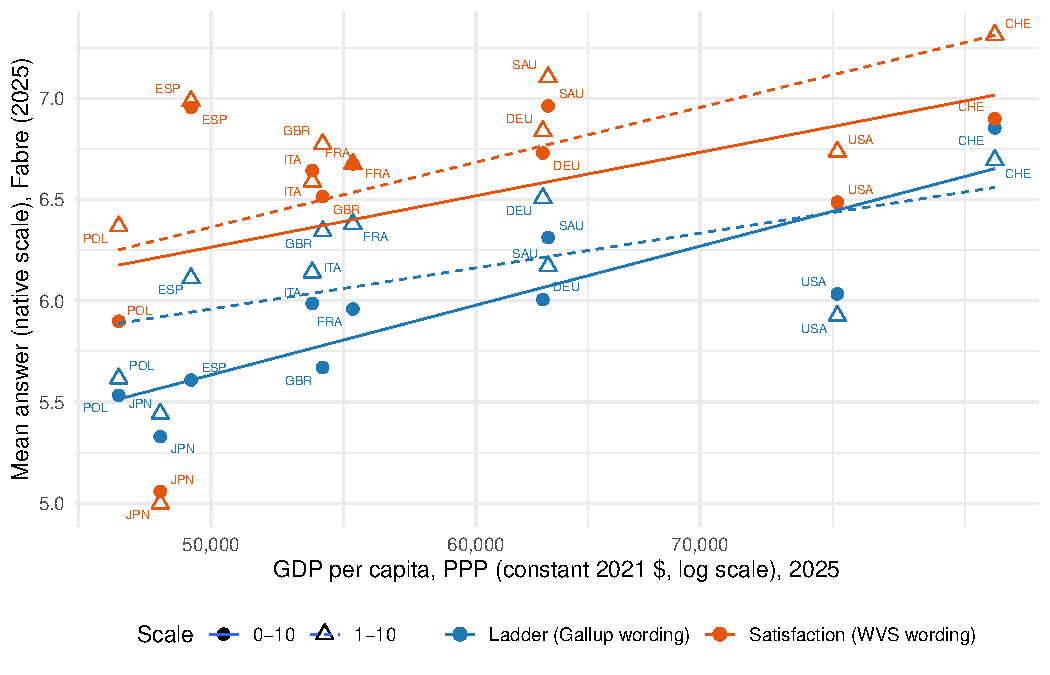
\includegraphics[width=.6\textwidth]{../figures/main/fabre_mean_vs_gdp_ppp.pdf}
    \caption{Mean life evaluation vs.\ GDP per capita (PPP, log scale) in ten countries, by randomized question variant (Fabre 2025, $n = \nFabre$). Colors: wording (Gallup's ladder or WVS life satisfaction); shapes and line types: scale (0--10 or 1--10). Mean answers on the native scale of each variant. Lines: OLS fits by variant.}\label{fig:fabre}
\end{figure}

The question also matters for levels. The ladder lowers answers by \effectLadder points on average (s.e.\ \seLadder) relative to the satisfaction question, which fully accounts for the lower level of Gallup answers in these countries: WVS answers exceed Gallup answers by \decompMeanGap points on average, and the question effect is \decompMeanQuestion points (SI Appendix, Table~S13). But the question effect does not explain why the gap varies across countries (share of the cross-country variance of the gap: \decompVarShareQuestion, 95\% CI [\decompLowVarShareQuestion; \decompHighVarShareQuestion]). Within countries, the wording does not affect the income gradient either: the interaction between the ladder wording and the respondent's income quartile is \interactionLadderIncome ($p \pInteractionLadderIncome$).

\subsection*{Neither survey is clearly more representative}

WVS samples over-represent tertiary-educated adults, by a median factor of \ratioTertiaryLow in countries with a GDP per capita below \$10,000, against \ratioTertiaryHigh above \$30,000, and over-represent urban residents in poorer countries (SI Appendix, Table~S15), as suspected by Deaton \citep{deaton_income_2008}. But correcting these imbalances has little effect: reweighting WVS samples to the population share of tertiary-educated adults changes the $R^2$ of mean satisfaction on log GDP only from \RtwoCommonWVSraw to \RtwoCommonWVSeduAdj, against \RtwoCommonGallupSub for Gallup in the same country-years. Gallup's centralized design is standardized, but it often uses only gender and age quotas, its samples are small, its microdata are not public, its modes changed during the pandemic, and part of its recent high-income interviews come from opt-in web panels \citep{gallup_methodology_2023}.

\section*{Discussion}

How much national income predicts well-being depends on the survey. In the WVS, GDP per capita explains a small share of the cross-country variance of well-being, less than a country's broad world region, because of large regional deviations: Latin America is happier, and Eastern Europe unhappier, than their income would predict. In the Gallup World Poll, income predicts as well as region. The experiment shows that both the question and the samples contribute to this discrepancy. Asked to the same respondents, the ladder is better predicted by GDP than life satisfaction, because life satisfaction produces larger country-specific deviations from the income gradient. Differences in wording reproduce about half of the difference in predictive capacity between the two surveys, the rest is attributable to the samples. %But the flat income gradient of the WVS is specific to its samples.

These results have implications for research. Cross-country conclusions about the income--well-being relationship, including rankings of the happiest countries, should be checked across surveys and questions, and the available evidence does not establish that either survey is more representative. The discrepancy is largest in low-income countries, which the experiment does not cover; replicating it face-to-face in low- and middle-income countries is the natural next step. The residual difference between surveys also lumps together sampling frames, modes, context and time, all of which can affect answers \citep{conti_survey_2011}, and which future designs could separate.

They also have implications for policy. Rich countries rarely have low life satisfaction, but middle-income countries can be as happy as the richest: the country-year with the highest mean happiness in the WVS is Kyrgyzstan in 2020, with a GDP per capita of about \$\gdpKGZ, and high life satisfaction is also reported in small-scale societies with very low monetary incomes \citep{galbraith_high_2024}. This echoes within-country evidence that income matters less for well-being than other life circumstances \citep{helliwell_hows_2003,blanchflower_well-being_2004,kahneman_would_2006}, although emotional well-being keeps rising with income for most people \citep{killingsworth_income_2023}. % and well-being rises with GDP within countries over time (SI Appendix, Table~S9). 
Growth thus does not appear necessary for high national well-being, which should be targeted directly \citep{stiglitz_report_2009,frijters_happy_2020}. Understanding the non-material factors behind regional differences---social ties, perceived freedom, culture, or response styles \citep{exton_comparing_2015,senik_french_2014}---is a priority.

\section*{Materials and Methods}

\paragraph{Well-being data.} I use the WVS time-series file \citep{wvs_trend_2022} (waves 1--7, 1981--2022), completed with the Joint EVS/WVS 2017--2022 dataset \citep{evs_wvs_joint_2024}, which adds the 2017 wave of the European Values Study and recent WVS surveys (\nWVSRespondents respondents, survey weights). As national averages of ordinal answers can be sensitive to how they are computed \citep{bond_sad_2019,kaiser_scientific_2022}, I compute eight national indicators from the happiness (4-point) and life-satisfaction (1--10) questions: the shares of happy, very happy and very unhappy people, their difference, mean happiness, mean satisfaction, the share satisfied (6--10), and the average of the shares happy and satisfied \citep{inglehart_genes_2000}. For Gallup, I use the distribution of ladder answers by country and year, tabulated from the World Poll microdata (\nGallupCountryYears country-years, 2006--2023), from which I compute the mean and six shares, and the three-year averages of the World Happiness Report \citep{whr_2026} for 2023--2025.

\paragraph{Income and regions.} Income is measured by GDP per capita at PPP (constant 2021 dollars) or at market exchange rates \citep{worldbank_wdi_2026}, in logs, in sextiles, or in $k$-means clusters ($k = 5$--7); missing values are imputed with IMF data \citep{imf_weo_2026} and growth rates. The main region classification follows the five UN regional groups: Africa, Asia (including the Middle East and Central Asia), Eastern Europe, Latin America, and Western countries. Robustness checks use six regions (isolating the Middle East), the World Bank regions, and six continents (SI Appendix).

\paragraph{Income vs.\ region.} For each indicator and income measure, I regress well-being on income, on region dummies, and on both, across country-years. The Shapley (LMG) share of the joint $R^2$ due to income is $s = [R^2_1 + (R^2_3 - R^2_2)]/(2R^2_3)$ \citep{lindeman_introduction_1980,gromping_estimators_2007}, where $R^2_1$, $R^2_2$ and $R^2_3$ are those of the three regressions; region is the better predictor if $s < 0.5$. Cross-validated $R^2$ predict each country's observations from a model estimated on all other countries. Robustness checks use each wave, population weights, the last observation per country, no EVS surveys, no pandemic years, no imputed GDP, an older GDP vintage, adjusted $R^2$, and alternative region classifications (SI Appendix, Table~S4).

\paragraph{Survey experiment.} The survey was conducted online by Bilendi (Kantar in Saudi Arabia) from April 15 to July 3, 2025, on \nFabre respondents in the United States, Japan, Saudi Arabia, Germany, the United Kingdom, France, Italy, Spain, Poland and Switzerland, with quotas on gender, age, income, education, region and urbanicity, and weights matching population frequencies. Toward the end of the questionnaire, each respondent was randomly assigned to one of four variants: the Cantril ladder (``Please imagine a ladder, with steps numbered from 0 at the bottom to 10 at the top\ldots'') or the WVS question (``All things considered, how satisfied are you with your life as a whole these days?''), with answers from 0 or from 1 to 10. The survey was approved by the CIRED institutional review board (IRB-CIRED-2025-2) %, respondents gave informed consent, 
and %the survey 
was pre-registered at \href{https://osf.io/7mzn4}{osf.io/7mzn4}. For the ten-country comparison, Gallup and WVS data are taken from the latest WVS/EVS survey of each country and the Gallup data of the same year (or at most three years apart). Confidence intervals come from 1,000 bootstrap replications resampling respondents within country and variant (experiment), within country (WVS), and answers within country (Gallup, multinomial draws). Individual-level estimates use OLS with country fixed effects and heteroskedasticity-robust standard errors.

\paragraph{Data and code availability.} Code and new data are available at \href{https://github.com/bixiou/wellbeing_gdp_region}{github.com/bixiou/wellbeing\_gdp\_region}. WVS and EVS data are freely available from the WVS Association and GESIS; Gallup World Poll data are proprietary and available from Gallup under license.

\paragraph{Acknowledgments.} I thank Claudia Senik, % whose 2016 assignment inspired this paper, % revision
participants in the 2024 STATEC Well-being Conference for helpful comments, Armon Rezai and the Vienna University of Economics and Business (WU Wien) for access to the Gallup World Poll data, and Julieta Toffoli for research assistance. This research received funding from Agence Nationale de la Recherche (ANR-24-CE03-7110). The author used Claude Opus 5.5 to write analysis code and draft parts of the manuscript, and reviewed and edited all content.

\paragraph{Author contributions.} A.F. designed research, performed research, analyzed data, and wrote the paper. \textbf{Competing interests:} The author declares no competing interest.

\bibliography{wellbeing}

\end{document}
